\documentclass{article}
\usepackage{graphicx,hyperref,amsmath,natbib,bm,url}
\usepackage{microtype,todonotes}
\usepackage[american]{babel}
\usepackage[a4paper,text={16.5cm,25.2cm},centering]{geometry}
\usepackage[compact,small]{titlesec}
\setlength{\parskip}{1.2ex}
\setlength{\parindent}{0em}
\clubpenalty = 10000
\widowpenalty = 10000
\usepackage{kpfonts}
\usepackage[T1]{fontenc}
\usepackage{float}

\begin{document}
\begin{center}
	\textbf{\Huge{Documentation of the Unit-tests}}
\end{center}

\section{GraphTester.java}
First it needs to be tested that all the methods a graph provides work as expected. These tests are implemented in the file "GraphTester.java".
\subsection{Empty constructor}
Name of the test: emptyConstructor() \\
After the call of the empty constructor a graph should exist. Furthermore, the graph's vertex set and edge sets should be of size 0 at this point. (There is one Hashtable "outEdges" with the index of the startvertex as key and the list of edges with this startvertex as values. The other Hashtable "inEdges" stores the edges with the endvertices as keys. The second Hashtable might be useful for further algorithms, that we did not implement.)

\subsection{Adding vertices}
\begin{itemize}
	\item Name of the test: testAddVertex() \\
	After the construction of a new vertex the vertex set should still be empty, since no vertex was added to the graph. \\
	The addition of some non-null vertex $v_0$ should be successful (which means that graph.add(v0) should return true). The vertex set should then contain the key 0 (since the vertex indices start at 0). And the size of the vertex set needs to be 1. This assures that no vertex other than $v_0$ is in the vertex set. \\
	A vertex with value null should not be added to a graph.
\end{itemize}

\subsection{Removing vertices}

\begin{itemize}	
	\item Name of the test: testRemoveVertex1()\\
	It should not be possible to remove a vertex in an empty graph.
	
	\item Name of the test: testRemoveVertex2()\\
	It should not be possible to remove a non-existent vertex in a non-empty graph.
	
	\item Name of the test: testRemoveVertex3()\\
	The test verifies that an existing vertex in a graph with one vertex can be removed.
	
	\item Name of the test: testRemoveVertex4()\\
	The test verifies that a existing vertex in a graph with more than one vertex can be removed as expected. Two vertices are added to the graph. One of them is removed afterwards and it is checked whether the removal was successful. It is tested whether the vertex which is not removed still exists in the vertex set.
	
\end{itemize}

\subsection{Adding edges}
\begin{itemize}
		\item Name of the test: testAddEdge1()\\
	An edge that contains a vertex with value null should not be added to the graph, so there are three cases tested:
	\begin{itemize}
		\item Adding an edge between two vertices with value null
		\item Adding an edge with exactly one vertex with value null (once the start vertex has value null, once the end vertex has value null)
		\item Adding an edge between two non-null vertices should, in contrast, be possible.
	\end{itemize}
	\item Name of the test: testAddEdge2() \\
	An edge that contains a vertex which is non-existent in the graph should not be added.
	\item  Name of the test: testAddEdge3() \\
	The test verifies that a correct edge is added. Six non-null vertices and six edges between them are added to a graph. Then it is tested whether all expected vertices and edges are contained in the vertex set and edge set, respectively.
	\item  Name of the test: testAddEdge4() \\
	The test checks that edges (which are correct according to testAddEdge3()) but have a weight < 0 are added to the graph. Their weight should be converted to 0. Here three boundary-cases are considered: (Remember that our software only supports integers as input for weights.)
	\begin{itemize}
		\item Adding an edge with weight 1
		\item Adding an edge with weight -1
		\item Adding an edge with weight 0
	\end{itemize}

	\item Name of the test: testAddEdge5()\\
	Verifies that a vertex can be part of more than one edge.
	\item Name of the test: testAddEdge5()\\
	An edge that already exists in the graph should not be added again, even if the weights are not the same.
\end{itemize}

\subsection{Removing edges}
\begin{itemize}
	\item Name of the test: testRemoveEdge1()\\
	The test verifies that when trying to remove an edge that contains a vertex with value null, no exception is thrown.
	\item Name of the test: testRemoveEdge2()\\
	In an empty graph no edge should be removed.
	\item Name of the test: testRemoveEdge2()\\
	A non-existing edge in a non-empty graph should not be removed.	
	\item Name of the test: testRemoveEdge3()\\
	The test verifies that an existing edge can be removed. First some vertices and edges are added. Then an edge is removed. The content of vertex set and edge set is tested to be as expected.
\end{itemize}	

\section{LoadingTest.java}
All types of input-files need to be considered. These tests are implemented in the file "LoadingTest.java". Please notice that if the method loadFile() in the DrawPanel returns false, there will be opened a window that informs the user about what went wrong. These windows can not be seen properly in the automated tests because they disappear too quickly. If you would like to check the error messages, please load the mentioned files directly via the program.
\subsection{Non-existent files}
Name of the test: notExistingFile()\\
The method loadFile() in the DrawPanel is supposed to throw a \emph{FileNotFoundException} if the given path does not exist. To test this, a DrawPanel is constructed (and tested to be not null). Then a non-existent file  "abc.txt" is tried to be loaded. A window should be shown that says that the file does not exist.
\subsection{Non- .txt files}
Name of the test: nontxtFile()\\
A file with a name that does not end with ".txt" should not be read in. No exception should be thrown in this case. A window should appear that says that you did not choose a .txt file.
\subsection{Files with duplicate edges}
Name of the test: duplicateEdge()
\begin{figure}[H]
	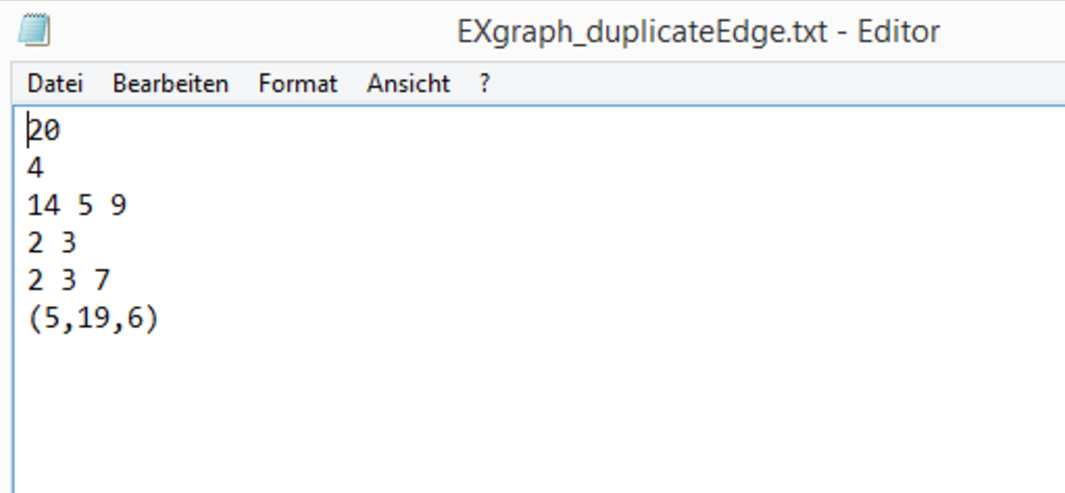
\includegraphics[width=.7\textwidth,keepaspectratio]{./img/duplicateEdge.pdf}
\end{figure}
The file "EXgraph\_duplicateEdge.txt" should be loaded. Since the edge (2,3) is contained twice, loadFile("EXgraph\_duplicateEdge.txt") should return false. Since the file should be read in, no exception should be thrown. It is tested that the other edges are added correctly.
\subsection{Files with incorrect number of edges}
Name of the test: lessEdges()
\begin{figure}[H]
	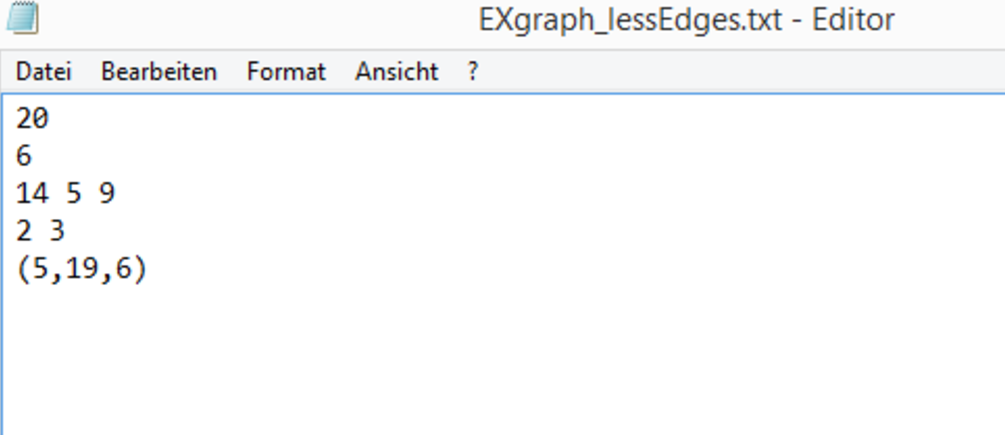
\includegraphics[width=.7\textwidth,keepaspectratio]{./img/lessEdges.pdf}
\end{figure}
The file should be loaded, so no exception should be thrown. Since there are only 3 edges given but it is stated that there are 6, loadFile("EXgraph\_lessEdges.txt") should return false. The graph should then contain the specified 19 vertices and 3 edges.
\subsection{Files in which the number of vertices or the number of edges is missing}
Name of the test: missingHead()
\begin{figure}[H]
	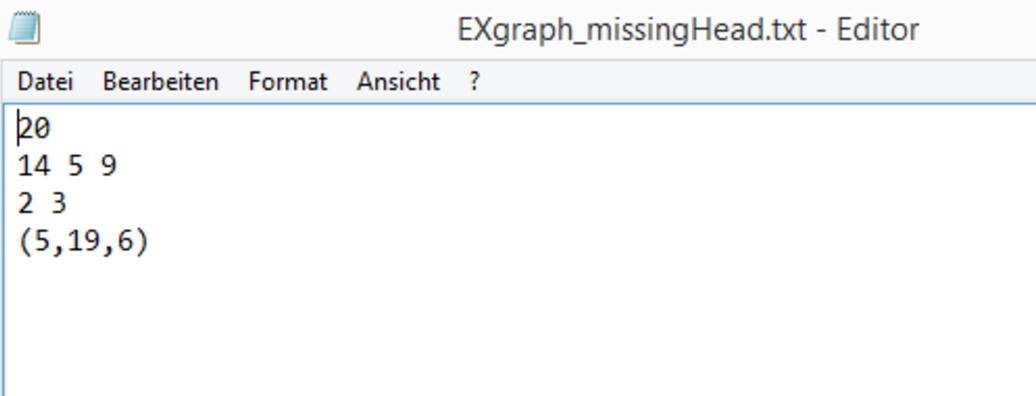
\includegraphics[width=.7\textwidth,keepaspectratio]{./img/missingHead.pdf}
\end{figure}
Since the file "EXgraph\_missingHead.txt" exists, no exception should be thrown. The load-method should return false. The graph should be empty because the number of vertices or the number of edges is not provided.
\subsection{Files that contain letters}
Name of the test: fileWithLetters()
\begin{figure}[H]
	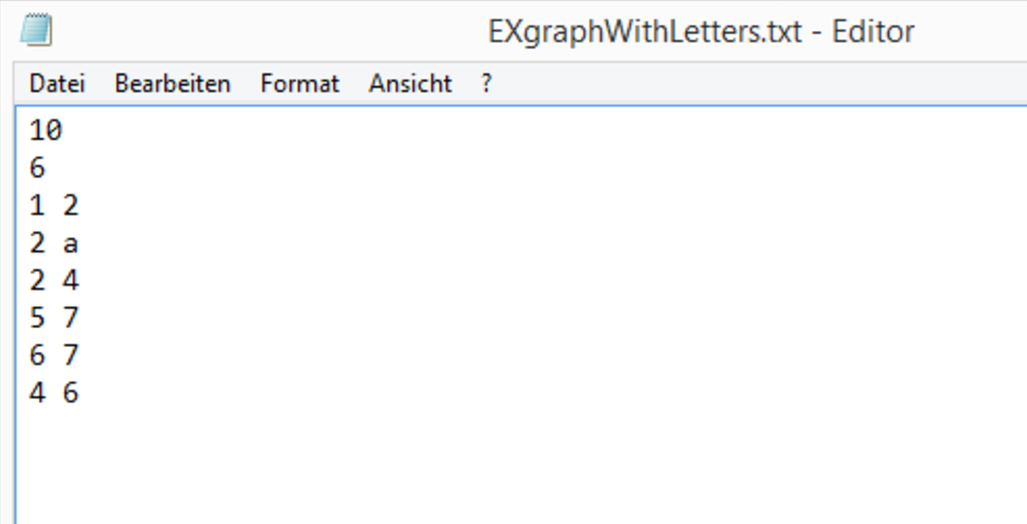
\includegraphics[width=.7\textwidth,keepaspectratio]{./img/letters.pdf}
\end{figure}
Since there is an edge that can not be read, the load-method should return false. The graph should just contain the other edges specified in the file. No exception should be thrown.
\subsection{Files with edges that are not in the correct format}
Name of the test: unreadableEdge()
\begin{figure}[H]
	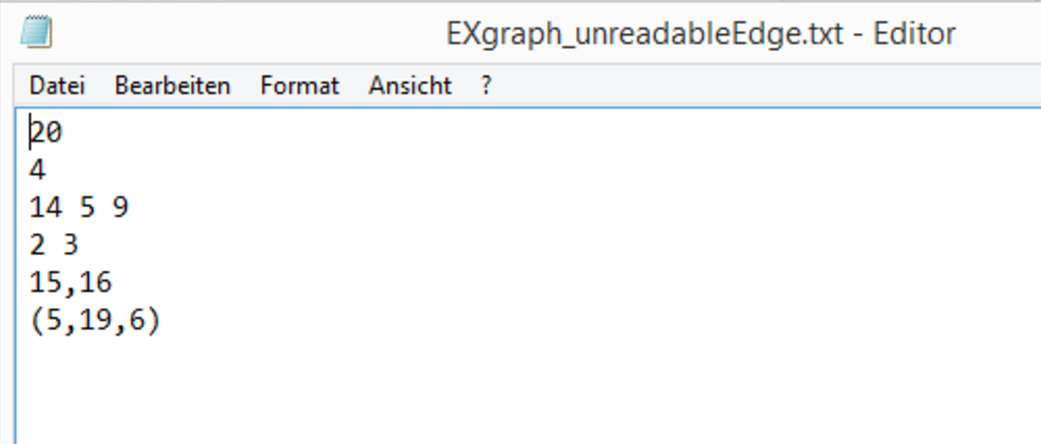
\includegraphics[width=.7\textwidth,keepaspectratio]{./img/unreadableEdge.pdf}
\end{figure}
The line "15,16" in the file "EXGraph\_unreadableEdge.txt" does not fit any edge type. Since the file exists, no exception should be thrown. The graph should only contain the other given edges.
\subsection{Empty file}
Name of the test: emptyFile() \\
This test assures that no error is thrown while reading an empty file. No vertices (and hence no edges) should be added to the graph.
\subsection{Files that are in the correct format}
Name of the test:readableGraph()
\begin{figure}[H]
	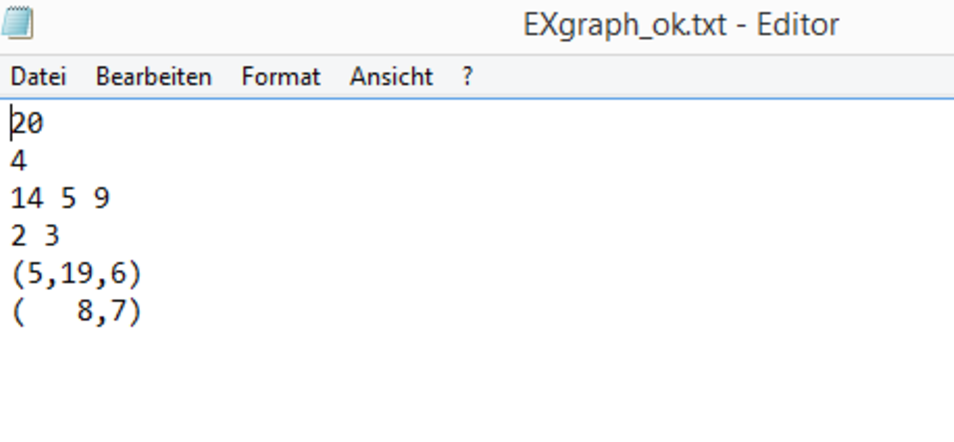
\includegraphics[width=.7\textwidth,keepaspectratio]{./img/EXGraphOk.pdf}
\end{figure}
To verify that files in the correct format are read in correctly, a file is read in that contains an edge for every supported edge-type. Note that space characters are ignored. It is checked that exactly all specified edges are contained in the graph.
\subsection{Files that contain edges with non-existent vertices}
Name of the test: edgeWithNonExistingVertex()
\begin{figure}[H]
	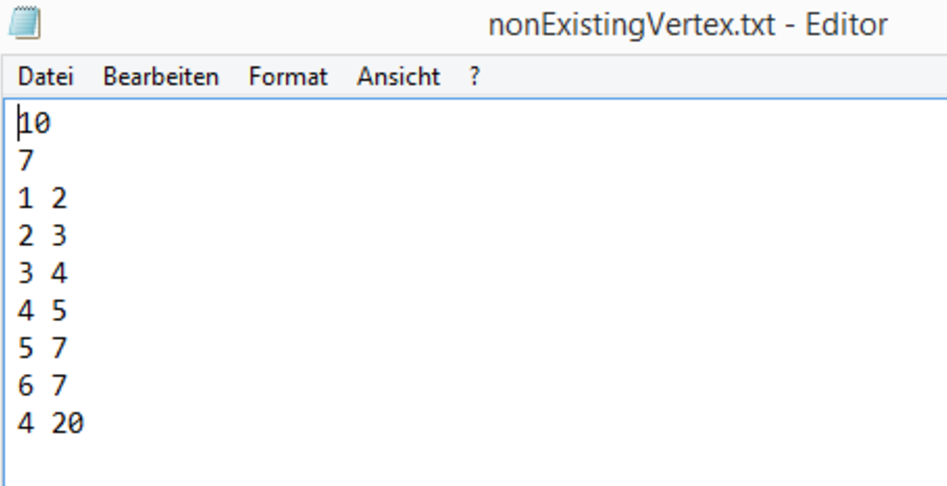
\includegraphics[width=.7\textwidth,keepaspectratio]{./img/nonExistingVertex.pdf}
\end{figure}
The last case tested is that a file that specifies an edge that contains a vertex which has an index $\geq$ the number in the first line. It should be recognized that such an edge can not be added to the graph. So the load-method should return false, but no exception should be thrown.

\section{ForceDirectedTester.java}
This class tests that a proper layout of the loaded files is found. We selected a file which specifies a graph that contains two cliques: One $K_3$ and one $K_4$ (and some isolated vertices):
\begin{figure}[H]
	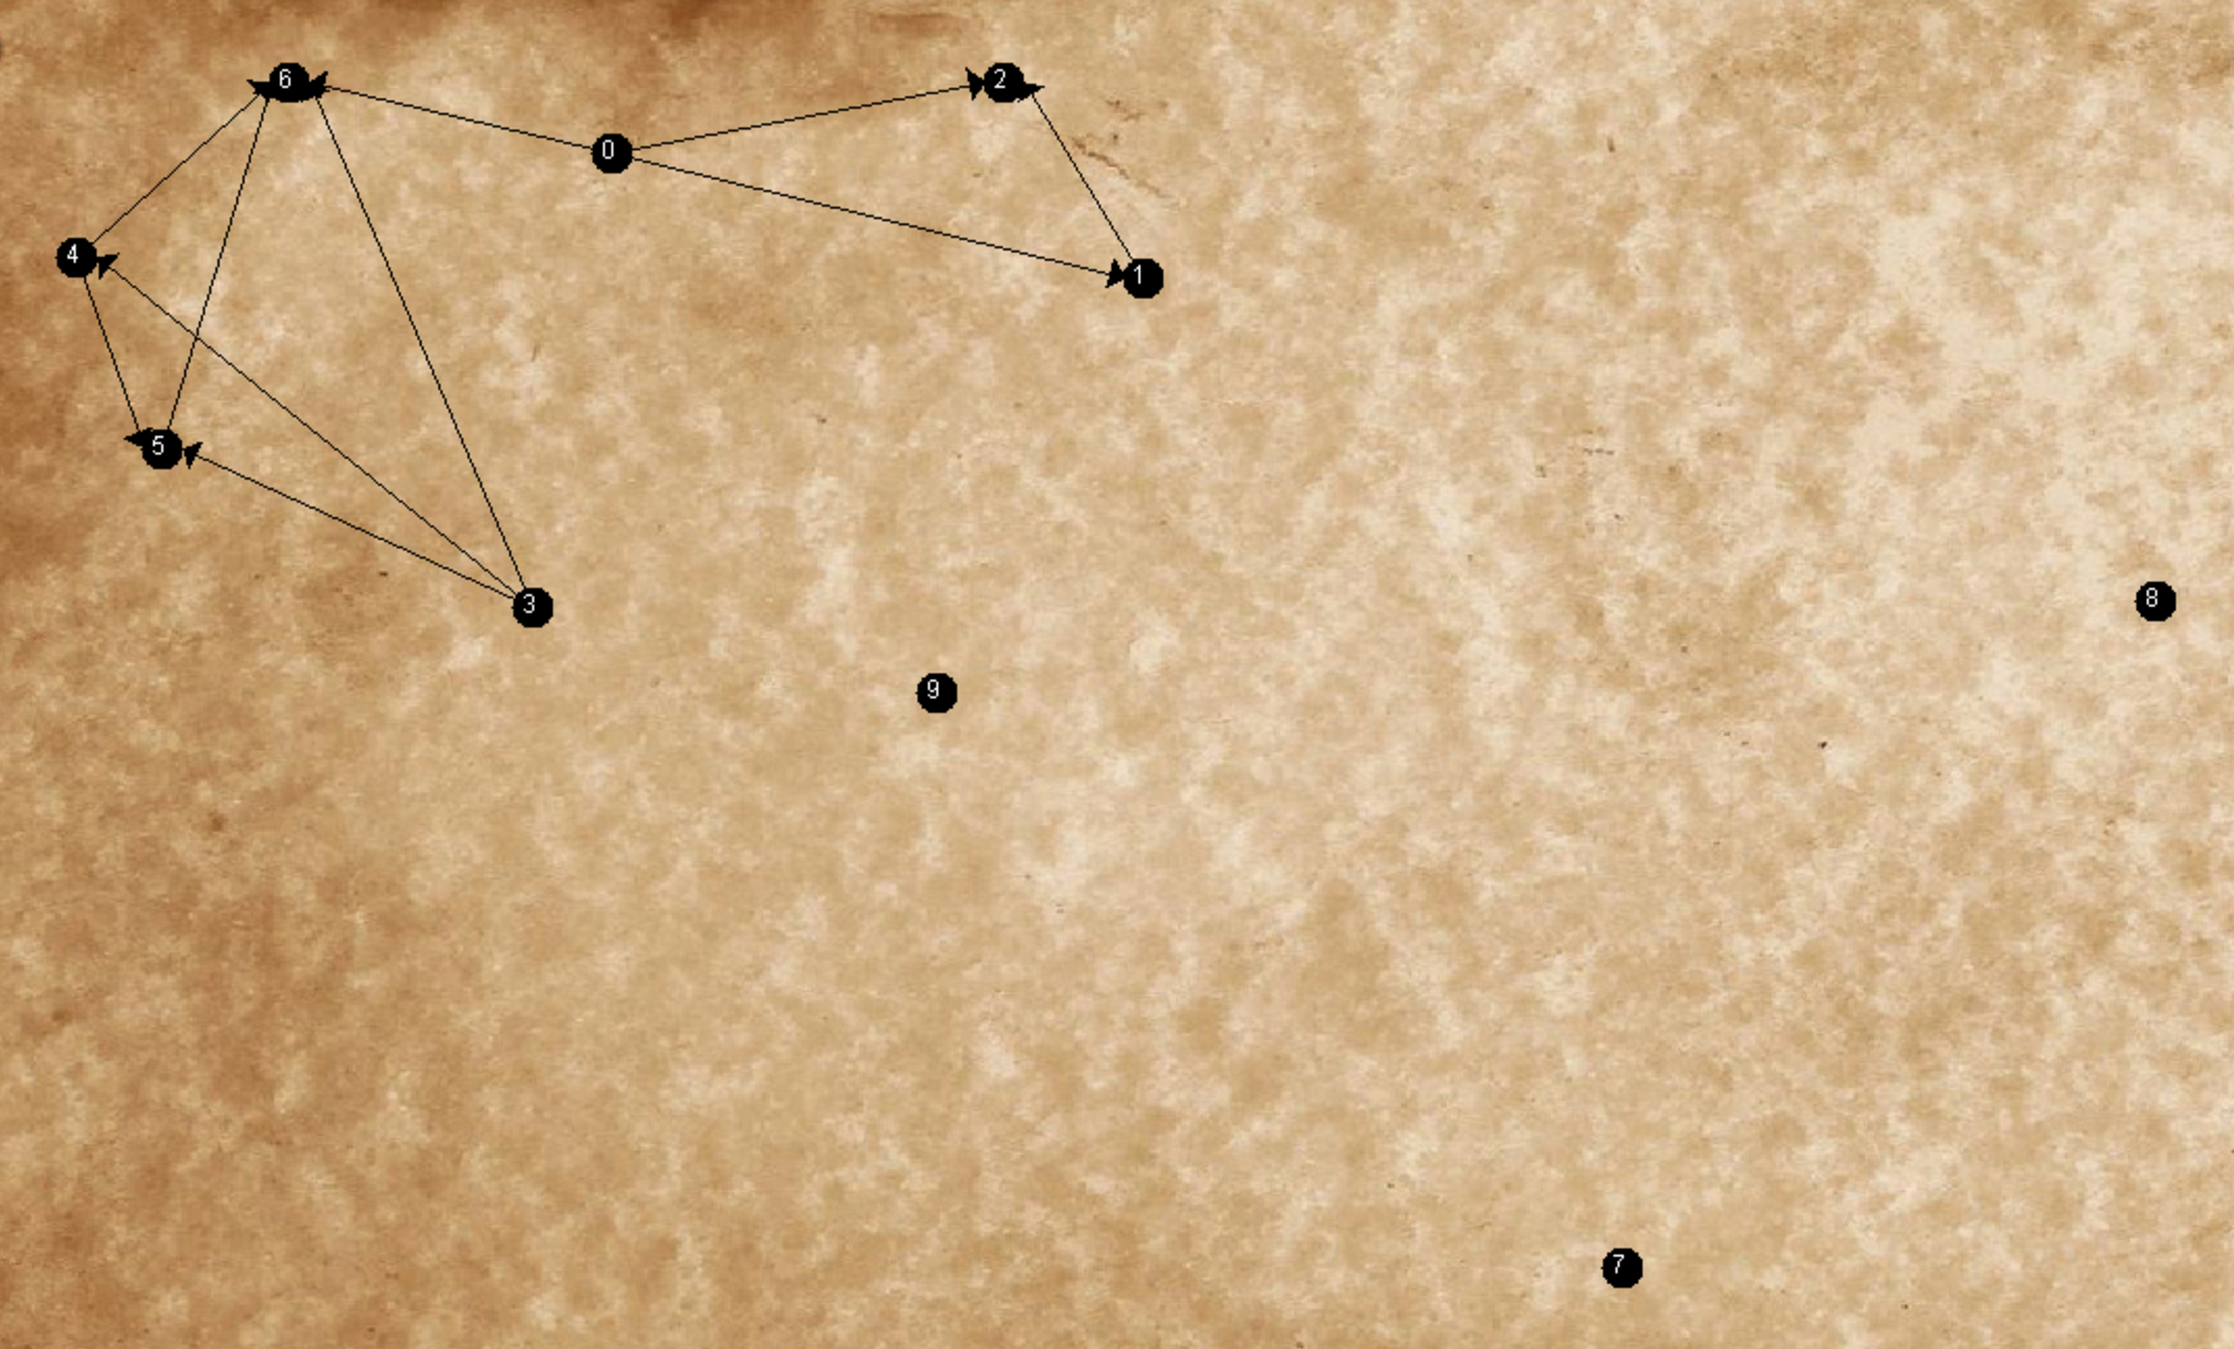
\includegraphics[width=\textwidth,keepaspectratio]{./img/forceDirected.pdf}
	\caption{This is how the loaded graph can look like. Please notice that the algorithm we chose is (pseudo-) non-deterministic. So the result and its quality can be different in each execution.}
\end{figure}
In the test the file "twoCliques.txt" is loaded. To verify that a proper layout was found, three averages are computed: The average distance "average1" between any pair of vertices within the $K_3$, the average distance "average2" between any pair of vertices within the $K_4$ and the "interCliqueAverage", which is the average distance between any vertex-pair $v,w$ with $v$ in $K_4$ and $w$ in $K_3$. It should hold that: \\
average1 < interCliqueAverage and average2 < interCliqueAverage \\
Since the algorithm we implemented is (pseudo-) non-deterministic, it makes sense to run this test multiple times. In some cases the test is not passed.

\section{Dijkstratester.java}
In all following tests the file "EXgraph.txt" is loaded:
\begin{figure}[H]
	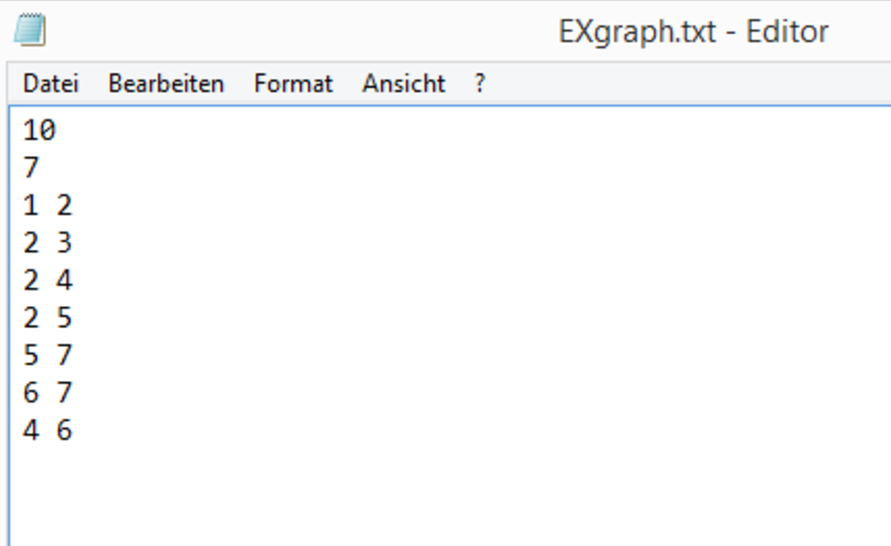
\includegraphics[width=.7\textwidth,keepaspectratio]{./img/EXGraph.pdf}
\end{figure}
The specified graph looks like this:
\begin{figure}[H]
	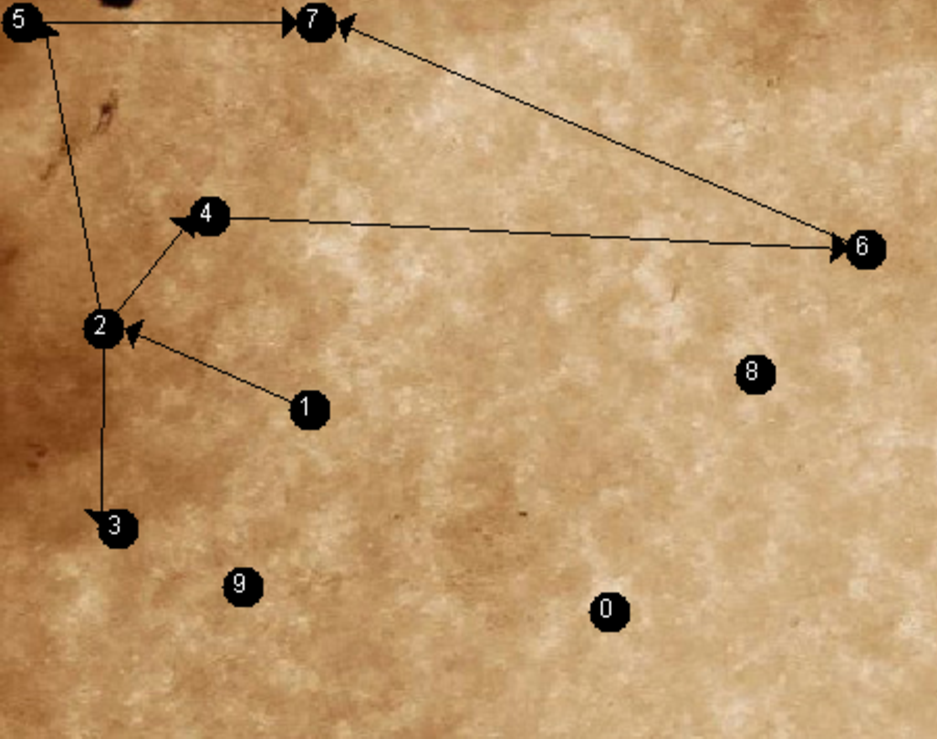
\includegraphics[width=.7\textwidth,keepaspectratio]{./img/drawPanel.pdf}
\end{figure}
\subsection{A path exists}
Name of the test: pathExists()\\
To test if an existing path is found, a new object of type interSteps is created which is supposed to find the path between vertex 1 and vertex 7. Then the Dijkstra is skipped to the end and the found path is compared to the expected sequence 7,5,2,1 (because it is saved backwards). The sequences should be equal.
\subsection{Input of non-existing vertices}
Name of the test: incorrectVertices()\\
There is no vertex with index 10. (If the user would click on the DrawPanel, that would be the next vertex to appear). Since there obviously is no path between vertex 1 and vertex 10, the path created like discribed above should be empty.
\subsection{Loops}
Name of the test: pathToItself()\\
This test verifies that the path from a vertex to itself is found and has weight 0. \\
After loading "EXgraph.txt" the edge (1,1) is added to the graph with weight 1. The path from 1 to itself should still consist of one entry and should still have weight 0.
\subsection{Isolated start vertex}
Name of the test: isolatedStart() \\
The vertex with index 0 is isolated, so there should be no path from vertex 0 to vertex 1.
\subsection{Isolated end vertex}
Name of the test: isolatedEnd() \\
Since vertex 0 is isolated, there should be no path from vertex 1 to vertex 0.
\subsection{No path and both vertices are not isolated}
Name of the test: noPath() \\
One boundary case to test is the situation where there is no path between two vertices with the additional restriction that they are both not isolated. In the graph we are currently looking at, this is the case for start vertex $v_5$ and end vertex $v_6$.

\subsection{Empty graph}
Name of the test: emptyGraph() \\
The special case that the graph is empty is tested in the file "DijkstraTester2.java". (Of course in this case "EXgraph.txt" is not loaded.) \\
It is arbitrarily tested that there is no path between "vertex 1" and "vertex 7".

\end{document}